\begin{pastexam}[label={px:ncku-107-prog-02}]{成大資訊聯招 107 學年度 第 2 題}
（問答）

(10\%) Compute the minimum weight spanning tree and it cost of the following graph.

\begin{center}
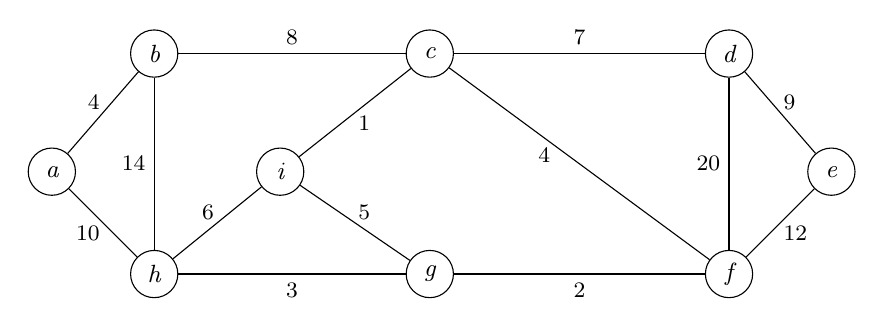
\begin{tikzpicture}[v/.style={circle,draw,inner sep=1pt,minimum size=6mm,font=\small\itshape},w/.style={inner sep=1pt,font=\footnotesize}]
\node[v] (a) at (0,1.5) {a};
\node[v] (b) at (1.3,3) {b};
\node[v] (h) at (1.3,0.2) {h};
\node[v] (i) at (2.9,1.5) {i};
\node[v] (c) at (4.8,3) {c};
\node[v] (g) at (4.8,0.2) {g};
\node[v] (d) at (8.6,3) {d};
\node[v] (f) at (8.6,0.2) {f};
\node[v] (e) at (9.9,1.5) {e};
\draw (a) -- node[w,above left] {4} (b);
\draw (a) -- node[w,below left] {10} (h);
\draw (b) -- node[w,left=2pt] {14} (h);
\draw (b) -- node[w,above=2pt] {8} (c);
\draw (c) -- node[w,below right] {1} (i);
\draw (c) -- node[w,above=2pt] {7} (d);
\draw (c) -- node[w,pos=0.4,below left] {4} (f);
\draw (i) -- node[w,above left] {6} (h);
\draw (i) -- node[w,above right] {5} (g);
\draw (h) -- node[w,below=2pt] {3} (g);
\draw (g) -- node[w,below=2pt] {2} (f);
\draw (d) -- node[w,left=2pt] {20} (f);
\draw (d) -- node[w,above right] {9} (e);
\draw (e) -- node[w,below right] {12} (f);
\end{tikzpicture}
\end{center}
\end{pastexam}

\begin{pastsoln}
答案：最小生成樹的邊是 $(c,i)$、$(f,g)$、$(g,h)$、$(a,b)$、$(c,f)$、$(c,d)$、$(b,c)$、$(d,e)$，
成本 $38$。 這張圖的最小生成樹只有一棵。

原題的 it cost 應是 its cost。 用 Kruskal 演算法（資結書第~24.2~節）：把邊依權重由小到大排，
依序檢查，兩端不在同一個元件裡就加進樹。 圖有 $9$ 個頂點，加滿 $8$ 條邊就停。 兩條權重 $4$ 的邊
先後順序不影響結果（兩條最後都會加進去）。

\begin{center}
\small
\begin{tabular}{clcl}
\toprule
步 & 邊（權重） & 加入？ & 加入後的元件（只列兩個以上頂點的） \\
\midrule
1 & $(c,i)$~1 & 是 & $\{c,i\}$ \\
2 & $(f,g)$~2 & 是 & $\{c,i\}$、$\{f,g\}$ \\
3 & $(g,h)$~3 & 是 & $\{c,i\}$、$\{f,g,h\}$ \\
4 & $(a,b)$~4 & 是 & $\{a,b\}$、$\{c,i\}$、$\{f,g,h\}$ \\
5 & $(c,f)$~4 & 是 & $\{a,b\}$、$\{c,f,g,h,i\}$ \\
6 & $(g,i)$~5 & 否 & $g$、$i$ 已在同一個元件（成環 $g$--$f$--$c$--$i$） \\
7 & $(h,i)$~6 & 否 & $h$、$i$ 已在同一個元件 \\
8 & $(c,d)$~7 & 是 & $\{a,b\}$、$\{c,d,f,g,h,i\}$ \\
9 & $(b,c)$~8 & 是 & $\{a,b,c,d,f,g,h,i\}$ \\
10 & $(d,e)$~9 & 是 & 全部 $9$ 個頂點，已有 $8$ 條邊，停 \\
\bottomrule
\end{tabular}
\end{center}

成本 $1 + 2 + 3 + 4 + 4 + 7 + 8 + 9 = 38$。 沒檢查到的 $(a,h)$~10、$(e,f)$~12、$(b,h)$~14、
$(d,f)$~20 都不在樹裡。 下圖粗線是樹邊，虛線是非樹邊。

\begin{center}
\begin{tikzpicture}[v/.style={circle,draw,inner sep=1pt,minimum size=6mm,font=\small\itshape},
    w/.style={inner sep=1pt,font=\footnotesize},
    te/.style={draw=memStroke, line width=1.6pt},
    ne/.style={draw=black!40, dashed}]
\node[v] (a) at (0,1.5) {a};
\node[v] (b) at (1.3,3) {b};
\node[v] (h) at (1.3,0.2) {h};
\node[v] (i) at (2.9,1.5) {i};
\node[v] (c) at (4.8,3) {c};
\node[v] (g) at (4.8,0.2) {g};
\node[v] (d) at (8.6,3) {d};
\node[v] (f) at (8.6,0.2) {f};
\node[v] (e) at (9.9,1.5) {e};
\draw[te] (a) -- node[w,above left] {4} (b);
\draw[ne] (a) -- node[w,below left] {10} (h);
\draw[ne] (b) -- node[w,left=2pt] {14} (h);
\draw[te] (b) -- node[w,above=2pt] {8} (c);
\draw[te] (c) -- node[w,below right] {1} (i);
\draw[te] (c) -- node[w,above=2pt] {7} (d);
\draw[te] (c) -- node[w,pos=0.4,below left] {4} (f);
\draw[ne] (i) -- node[w,above left] {6} (h);
\draw[ne] (i) -- node[w,above right] {5} (g);
\draw[te] (h) -- node[w,below=2pt] {3} (g);
\draw[te] (g) -- node[w,below=2pt] {2} (f);
\draw[ne] (d) -- node[w,left=2pt] {20} (f);
\draw[te] (d) -- node[w,above right] {9} (e);
\draw[ne] (e) -- node[w,below right] {12} (f);
\end{tikzpicture}
\end{center}

\textbf{為什麼只有一棵。} 由資結書推論~24.11，只要檢查每條非樹邊都比它在樹上兩端之間路徑的
最大權重\textbf{嚴格}大：
\begin{itemize}
\item $(g,i)$~5：樹上路徑 $g$--$f$--$c$--$i$，最大 $4$。
\item $(h,i)$~6：樹上路徑 $h$--$g$--$f$--$c$--$i$，最大 $4$。
\item $(a,h)$~10：樹上路徑 $a$--$b$--$c$--$f$--$g$--$h$，最大 $8$。
\item $(e,f)$~12：樹上路徑 $e$--$d$--$c$--$f$，最大 $9$。
\item $(b,h)$~14：樹上路徑 $b$--$c$--$f$--$g$--$h$，最大 $8$。
\item $(d,f)$~20：樹上路徑 $d$--$c$--$f$，最大 $7$。
\end{itemize}
都成立，所以這是唯一的最小生成樹。 用 Prim 演算法（資結書第~24.3~節）從任何頂點開始，也會得到
同一棵樹、同樣的成本 $38$。
\end{pastsoln}
